\documentclass[19pt,a4paper]{article}
\usepackage{xeCJK}
\usepackage{amsmath}
\setmainfont{STSong}
\usepackage{geometry}
\geometry{left=2.5cm,right=2.5cm,top=2.5cm,bottom=2.5cm}
\setlength{\parindent}{4em}
\usepackage{graphicx}
\title{第一次实验报告}
\author{王诗俊2015201951\quad 廖钰蕾2015201953\quad  孟妍廷2015202009\quad  刘笑2015201925}
\date{2017年10月7日}

\begin{document}
\maketitle

\textbf{一\quad 准备过程:}\\
\indent 首先按照老师的ppt在淘宝上购买材料(由于按照ppt上的链接来买,漏买了杜邦线和面包板)\\
\indent 参考了淘宝店的安装教程\\
\begin{figure}[htbp]
 \centering
 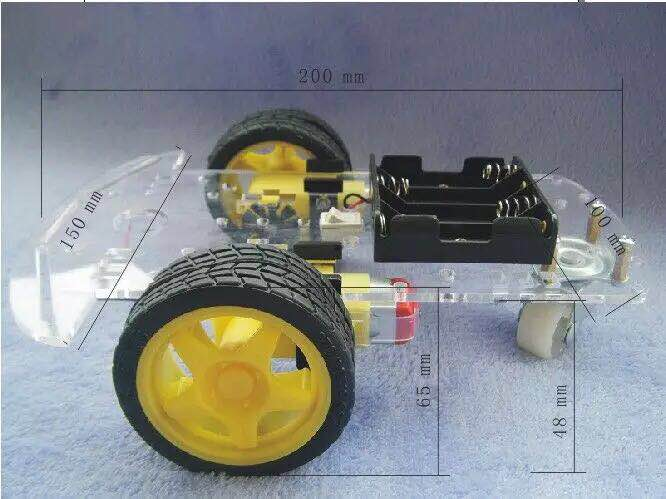
\includegraphics[scale=0.4]{2.jpeg}
\end{figure}\\

\indent 研究了arduino论坛上的高手的教程
\\
\\
\indent\textbf{二\quad 遇到的问题及解决;}\\ 
\indent 1.没有面包板、杜邦线和面包线(国庆期间不发货。。。)\\
\indent\ \ 找其他小组借到了并开始组装 \\
\\
\indent 2.小车的固定板和轮子的固定板尺寸不匹配\\
\indent\ \ 用裁纸刀手动裁切到合适的尺寸\\
\\
\indent 3.小车的轮子不是正圆且大小不一样,左右马达转速不同\\
\indent\ \  我们事先准备了两套小车的套件,将四个轮子进行反复测试挑选出与马达最适合的两个\\
\\
\indent 4.缺乏UNO板和电机驱动马达板的接线的知识\\
\indent\ \ 为了了解接线原理,我们参考了很多文献,主要文献如下:\\
\indent\ \    http://blog.csdn.net/keysking/article/details/54783046\\
\indent\ \    http://www.cnblogs.com/rayray/p/3157601.html\\
\\
\indent 5.上传代码出现问题\\
\indent\ \ 一位队友的电脑缺少插件无法上传代码进UNO板中,换了一台电脑后,在调试时仍然出现无\\
\indent 法上传的情况,经过检查发现是由于0-1口被杜邦线占用无法进行数据传输,拆除线后解决了问\\
\indent 题.\\
\\
\\
\\
\indent\textbf{三\quad 成果展示;}\\
\begin{figure}[htbp]
 \centering
 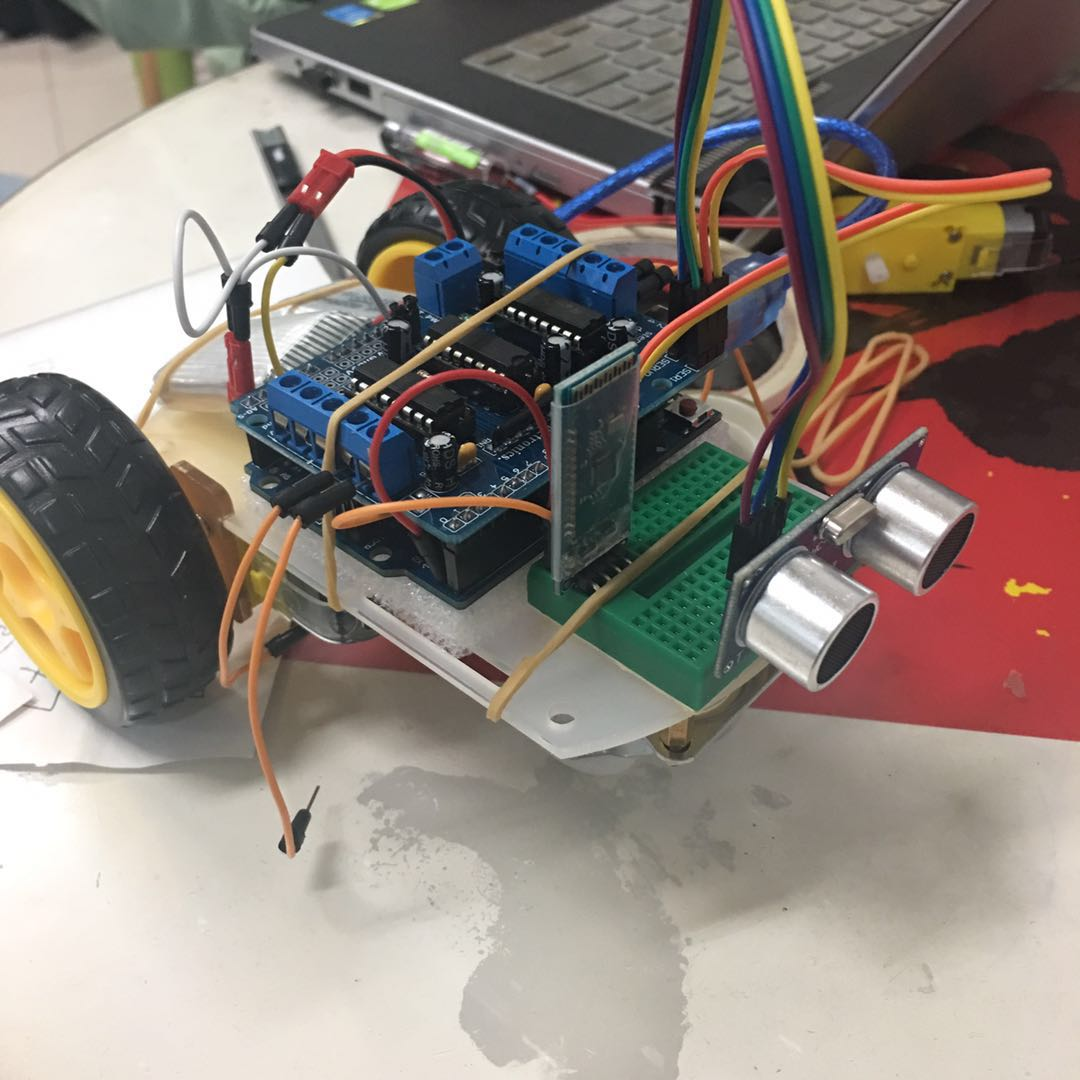
\includegraphics[scale=0.2]{1.jpeg}
\end{figure}\\
\indent 实现了小车遇到障碍物自动右转,手动控制小车左转、右转、前进、后退和停止。\\
\indent 具体展示见视频\\
\end{document}